\documentclass{article}
\usepackage{graphicx} % Required for inserting images
\usepackage{amsmath}
\usepackage{amssymb}
\usepackage{hyperref}
\usepackage[font=small,labelfont=bf]{caption} % Required for specifying captions to tables and figures

\title{Project 2 - Encrypted covert channel}
\author{Felix Mölder - au737970}
\date{March 2024}

\begin{document}
\maketitle
We want to create an encrypted secret channel between a client and a server that uses ICMP packets to hide the traffic. Thus, we have two programs. One for the client and one for the server. Attached you can find screenshots of the channel and wireshark.

\section*{Client:}

The client program first asks for input. Then the input is encrypted using AES in CBC mode. The key is saved in a separate file (secret\_client.py) and imported at the beginning of the program. To send a proper ICMP packet, we need to add a header to the ciphertext. This header has a size of 8 bytes and contains the ICMP type (1 byte), the ICMP code (1 byte) and the checksum (2 bytes). Furthermore, it contains an identifier (2 bytes) and a sequence number (2 bytes). The last four bytes depending on the type, but since we use type 47, we have these two fields. Thus, we know:
\begin{itemize}
    \item[type:] 47
    \item[code:] 0
    \item[checksum:] ?
    \item[identifier:] process identifier
    \item[sequence number:] 0      
\end{itemize}
The identifier can be obtained by using the getpid method of the os package. It is used to distinguish different ICMP packets but since we use type 47 (very uncommon), it is unlikely that other ICMP packets occur and therefore the process id is not relevant similar to the sequence number which we set to 0. The checksum is calculated by creating a dummy header with the value 0 as the current checksum and calculate by the given function (calculate\_checksum). This function was used from \href{https://github.com/00dhkim/icmp-tunneling-tool/blob/master/pyping/core.py}{icmp tunneling tool}. Once we have such a proper checksum, we create the final header with this and put the header and the ciphertext together as a packet. Finally, we create a raw socket and send the packet to the destination IP address given as a first argument. To run the file execute: "sudo python client.py '127.0.0.1'". 

\section*{Server:}

The server program first creates an ICMP socket and listens on the network layer. For each ICMP package the function recvfrom of the socket package extracts the source IP address and the package content (header + payload). Th first 20 bytes are the IP header and not interesting for us. The bytes 20 to 28 are the ICMP header and the rest is the payload. We struct the ICMP header in type, code, checksum, process id and sequence number. If the type is 47, the program decrypts the payload of the package with the same algorithm and the same secret key (secret\_server.py) and prints the source IP address followed by the plaintext. The program can be started by the command: "sudo python server.py". 

\section*{Appendix}

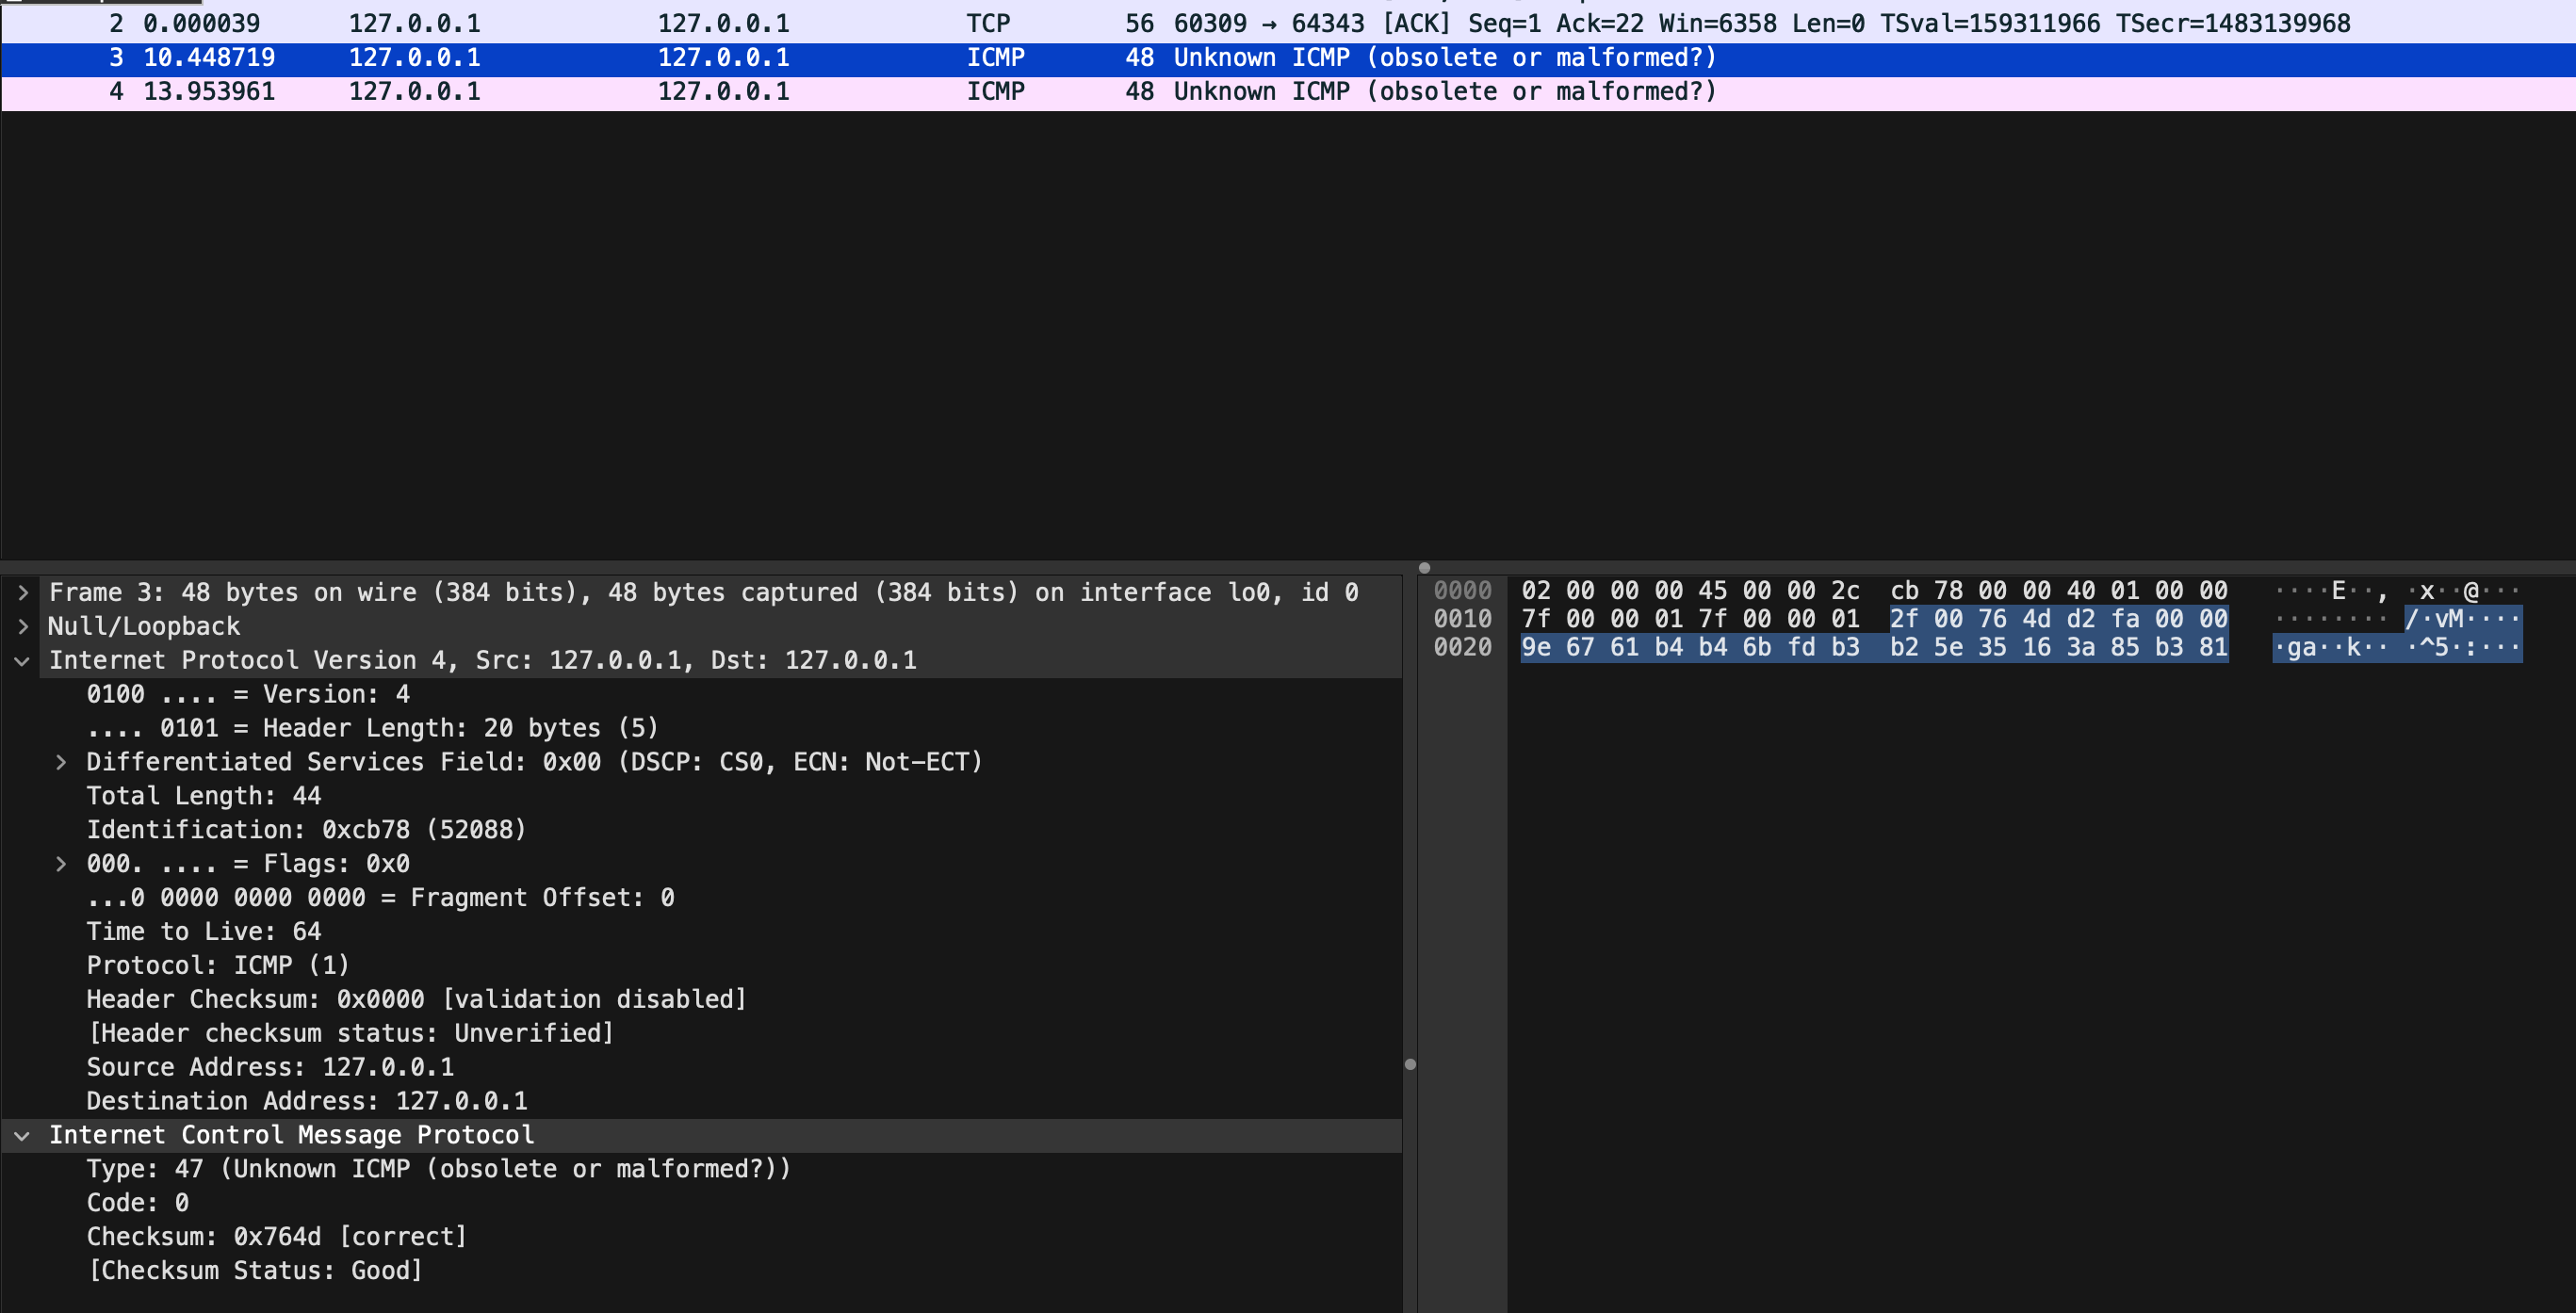
\includegraphics[width=\textwidth]{Wireshark}
\captionof{figure}{Wireshark capture of ICMP package}
$\newline$
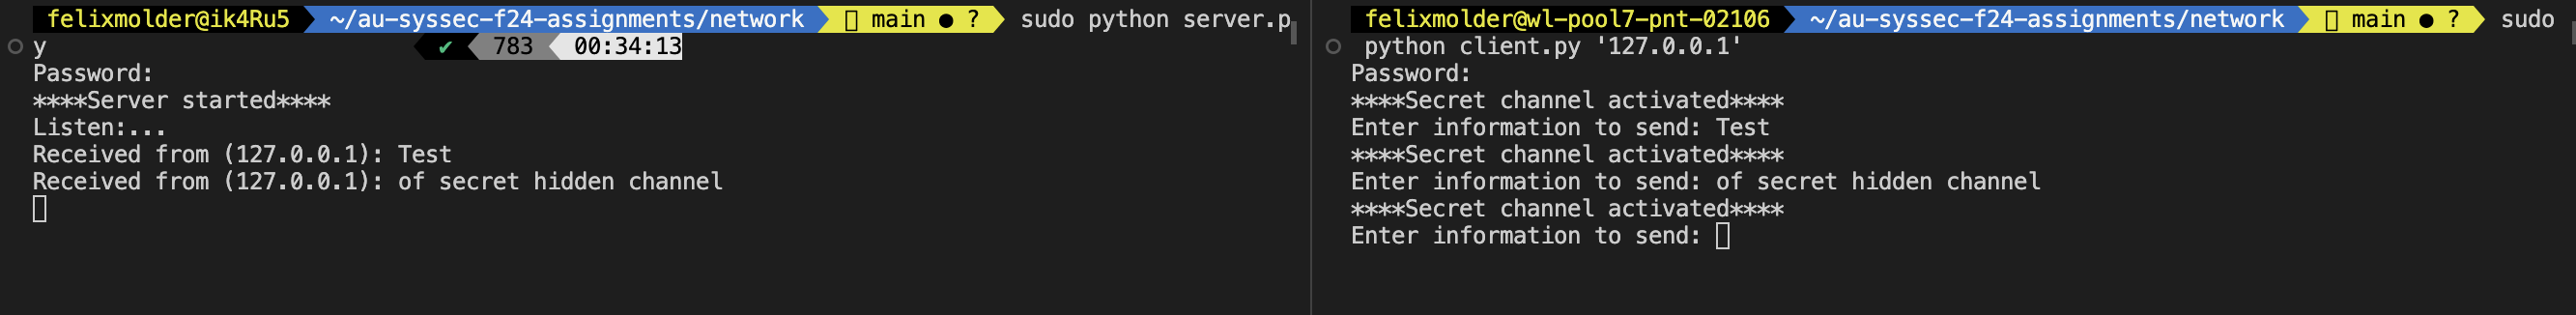
\includegraphics[width=\textwidth]{Terminal}
\captionof{figure}{Terminal of the conversation between client and server}
\end{document}